\section{Experimental Setup}

\subsection{Environments with Evolving Objectives}
We begin by describing the multi-objective environments that we evaluate our framework on. Despite their practical relevance, environments with multiple evolving objectives have received little attention in the multi-objective RL literature.

\textbf{Coffee Shop.}\quad We implement a simple but challenging gridworld environment which consists of an \(n \times n\) grid with \(m\) targets that are moving at a small rate and stochastically change directions. Each target stays alive for a certain number of timesteps before which the agent has to reach it. Once the target expires or the agent reaches it, another new target immediately respawns at a random position in the grid. The metric the agent has to maximize is the difference between the number of targets reached and the number of targets that expired. This flexible environment also allows us to introduce more targets at deployment time.

\begin{figure}[h]
  \centering
  \begin{subfigure}[t]{0.4\textwidth}
    \centering
    
\includegraphics[width=\linewidth]{img/grid_preview.png}
    \caption{Coffee Shop}
  \end{subfigure}
  \qquad
  \begin{subfigure}[t]{0.3\textwidth}
    \centering
    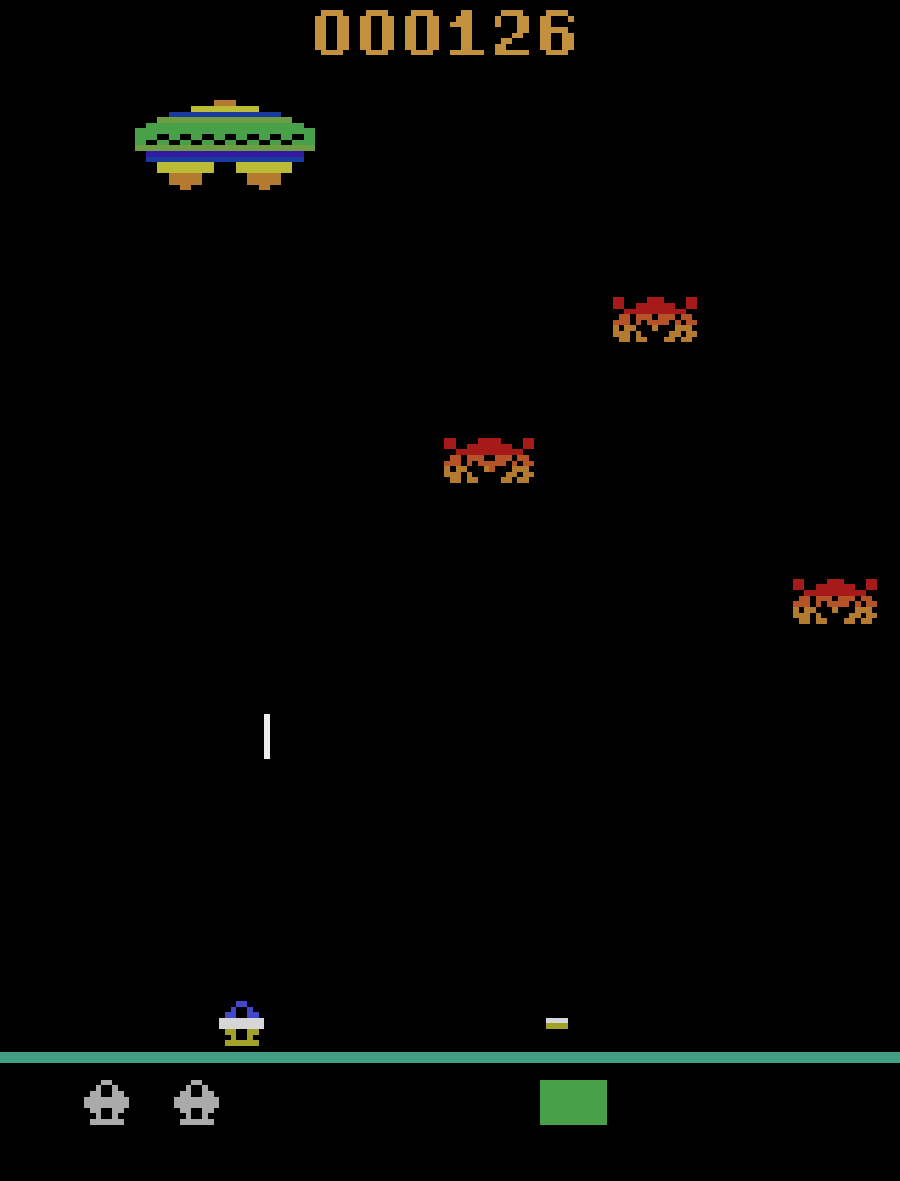
\includegraphics[width=\linewidth]{img/assault_preview.png}
    \caption{Atari Assault}
  \end{subfigure}
  \caption{Preview of the two evaluation environments.}
\end{figure}

In our experiments, we choose a \(30 \times 30\) grid with \(8\) targets. The observations for all the local policies includes information about all the targets (positions and expiry times) and the agent; but they are reordered so that the specific target of a policy is present at the first index. This enables sharing the same actor network across policies. When the agent reaches a target before the expiration, we reward the corresponding policy and penalize it if not. Both the reward and the penalty are equal in magnitude. Furthermore, we include a distance based reward shaping for each policy with respect to its target which is crucial to the learning. \todo{Include this as an advantage of our framework in introduction because there is no sensible reward shaping we can do in a single-policy approach.}

\textbf{Atari Assault.}\quad We also test our method on the Atari game Assault in which we control a missile and shoot alien ships that move. Even though this is not seen as a multi-objective environment, we decompose it so that we can treat each alien ship as a different objective. Since these alien ships move around and there are a variable number of ships at any point of time, it is a perfect testbed for our modular approach. We check whether we can synthesize interpretable policies that split control of the missile to target different ships. However, as the standard Atari games from the Arcade Learning Environment \citep{bellemare13arcade} either use image or raw RAM observations, we cannot decompose the game score and design rewards for the multiple policies. Instead, we turn to the Object-Centric Atari environments \citep{delfosse2023ocatari} which exposes object positions and states by decoding RAM states. This permits us to design decomposed observations and rewards for each policy to pursue and shoot the alien ships. However, the metric we optimize is still the game score.

The observation space consists of the positions of the cannon, the alien ships and enemy missiles, current health level, and the number of remaining lives. Similar to Dynamic Targets, we reorder the positions of the alien ships in the observations for each policy. Instead of rewards based on the game score, we design the rewards for each policy. We reward a policy if it successfully destroys an alien ship and penalize it if it loses a life. \todo{Also talk about how each policy needs to learn to evade alien missiles.}

\subsection{Baseline Approaches}

We compare our method against two baselines: a single policy PPO with weighted rewards and deep W-learning (DWN; \citet{rosero2024multi}). 
For the PPO baseline, since all the objectives have the same importance across the two environments, we use the total reward across objectives at each step as the reward function. 
The observation space remains the same as the multi-policy setting. 
However, we do not implement any reward shaping for the Dynamic Targets environment due to the difficulty of specifying a meaningful dense reward signal in the presence of multiple targets. 
We borrow the PPO implementation from CleanRL~\citep{huang2022cleanrl}.
We use the specified PPO hyperparameters from CleanRL for Atari Assault and we tune the hyperparameters for the Dynamic Targets environment with 40 Optuna iterations~\citep{akiba2019optuna}.

DWN is another multi-policy method for multi-objective RL that uses DQN for each of the local policies and additionally learns a W-network for each policy that predict scalar weights. 
These weights are used to choose which policy's action should be played at each step. 
The W-network is trained alongside the Q-network by updating it with a gradient step to predict the negative TD-error when the policy does not get to play its action.
The assertion here is that the negative TD-error quantifies how important it is for the policy to play its action. 
The implementation is borrowed from their repository.